%ATTENZIONE: PER COMPILARE BISOGNA FARE A MANO
%dvipdf tensor.dvi ;mv tensor.pdf temp.pdf 
%Dovremmo forse aggiungere due parole sulle C* algebras: non sono stateintrodotte proprio per evitare il tensor product in infinitedimensional systems?
%%%%%%%%%%%%%%%%%%%%%%%%%%%%%%%%%%%%%%%%%%%%%%%%%%%%%%%%%%%%%%%%%%%%%%%%
% The four postulates of quantum mechanics are three
%%%%%%%%%%%%%%%%%%%%%%%%%%%%%%%%%%%%%%%%%%%%%%%%%%%%%%%%%%%%%%%%%%%%%%%%
\documentclass[aps,prl,amsmath,amssymb,twocolumn,nofootinbib]{revtex4}
%\documentclass[twocolumn,aps,showpacs,prl,groupedaddress]{revtex4}
%\usepackage{amssymb,stackengine}
\usepackage{amssymb}
\usepackage{color}
\usepackage{graphicx}
\usepackage{epsfig,amssymb,amsmath,amsthm}
%\usepackage[active]{srcltx}
%\usepackage[hypertex,linkcolor=red]{hyperref}

\usepackage{color}
\usepackage{cancel}
\usepackage{tikz-cd}

\theoremstyle{plain}
\newtheorem{thrm}{Theorem}[section]
\newtheorem{form}[thrm]{Formalization}
\newtheorem{prop}[thrm]{Proposition}
\newtheorem{lem}[thrm]{Lemma}

\theoremstyle{definition}
\newtheorem{defn}[thrm]{Definition}
\newtheorem{post}{Postulate}[]
\renewcommand*{\thepost}{(\alph{post})}

\theoremstyle{remark}
\newtheorem*{remark}{Remark}


\newcommand{\blue}{\color{blue}}  %NON LINEAR
\newcommand{\red}{\color{red}}
\newcommand{\cyan}{\color{cyan}}
\newcommand{\green}{\color{green}} %THEORY quantum state estimation
\newcommand{\yellow}{\color{yellow}} %THEORY quantum channel estimation

\DeclareMathOperator{\spn}{span}

\newcommand{\pj}[1] {\underbar{$#1$}}
%\newcommand{\pj}[1] {\overline{#1}}

\def\>{\rangle}
\def\<{\langle}
\def\ca{_{\cal A}}
\def\cb{_{\cal B}}
\def\cc{_{\cal C}}
%\def\comment#1{}
\def\comment#1{ [{\bf Comment Lor:} {\sf #1}]}
\def\commentg#1{ [{\bf Comment Gabriele:} {\sf #1}]}
\def\labell#1{\label{#1}}
%\def\labell#1{\label{#1}{\mbox{{\tiny #1}}}}
%\def\section#1{{\par\em #1:--- }}
\def\togli#1{}
\def\sh{\mbox{sh}}
\def\iden{\openone}
\begin{document}

%\fbox{{\scriptsize Preprint. \today}}
\title{The four postulates of quantum mechanics are three}
\author{Gabriele Carcassi$^1$, Lorenzo Maccone$^{2,*}$ and Christine A. Aidala$^1$
}\affiliation{\vbox{1.~Physics Department, University of Michigan, 450 Church Street,
	Ann Arbor, MI 48109-1040,
	United States}\\
  \vbox{2.~Dip.~Fisica and INFN Sez.\ Pavia, University
    of Pavia, via Bassi 6, I-27100 Pavia, Italy}}
\begin{abstract}
  The tensor product postulate of quantum mechanics states that the
  Hilbert space of a composite system is the tensor product of the
  components' Hilbert spaces. All current formalizations of quantum
  mechanics that do not contain this postulate contain some equivalent
  postulate or assumption (sometimes hidden). Here we give a natural
  definition of composite system as a set containing the component
  systems and show how one can logically derive the tensor product
  rule from the state postulate and from the measurement postulate. In
  other words, our paper reduces by one the number of postulates
  necessary to quantum mechanics.
\end{abstract}
\pacs{}
% Measurement theory (quantum mechanics), 03.65.Ta Mechanics quantum,
% 03.65.-w noise quantum, 42.50.Lc quantum information, 03.67.Ac
% Quantum information, 03.67.-a Quantum fluctuations, 42.50.Lc quantum
% mechanics, 03.65.Ta quantum optics, 42.50.Gy
\maketitle


The tensor product postulate does not appear in all axiomatizations of
quantum mechanics: it has even been called ``postulate 0'' in some
literature \cite{zurek}. A widespread belief is that it is a direct
consequence of the superposition principle, and it is hence not a
necessary axiom. {\em This belief is mistaken}: the superposition
principle is encoded into the quantum axioms by requiring that the
state space is a {\em linear} vector space. This is, by itself,
insufficient to single out the tensor product, as other linear
products of linear spaces exist, such as the direct product, the
topological product or the direct sum of vector spaces, which are used
in classical mechanics to combine state spaces of linear systems.
This belief may have arisen from the seminal book of Dirac
\cite{diracbook}, who introduces tensor products (Chap.~20) by
appealing to linearity. However, he adds the seemingly innocuous
request that the product among spaces be distributive (rather,
bilinear), which is equivalent to postulating tensor products (or
linear functions of them). This is not an innocuous request. For
example it does not hold where the composite vector space of two
linear spaces is described by the direct product, e.g.~in classical
mechanics, for two strings of a guitar: it is not distributive.
[General classical systems, not only linear ones, are also composed
through the direct product.] Of course, Dirac is not constructing an
axiomatic formulation, so his `sleight of hand' can be forgiven. In
contrast, von Neumann (\cite{vonneumannbook} Chap.~VI.2, also
\cite{jauch}) introduces tensor products by noticing that this is a
natural choice in the position representation of wave mechanics (where
they were introduced in \cite{weyl,epr}), and then {\em explicitly
  postulates} them in general: ``This rule of transformation is
correct in any case for the coordinate and momentum operators [...]
and it conforms with the [observable axiom and its linearity
principles], we therefore postulate them generally.''
\cite{vonneumannbook}.  More mathematical or conceptually-oriented
modern formulations (e.g.~\cite{ozawa,masanes,wootters,nielsenchuang})
introduce this postulate explicitly.  An interesting alternative is
provided in \cite{ballentinebook,ballentinepaper}: after introducing
tensor products, Ballentine verifies a posteriori that they give the
correct laws of composition of probabilities. Similarly, Peres uses
relativistic locality \cite{peres}. While these procedures seemingly
bypass the need to postulate the tensor product, they do not guarantee
that this is the {\em only} possible way of introducing composite
systems in quantum mechanics. In the framework of quantum logic,
tensor products arise from some additional conditions \cite{matolcsi}
which (in contrast to what is done here) are not connected to the
other postulates. A similar approach was followed in \cite{aerts}
where tensor products were obtained by specifying some additional
physical requirements. In quantum field theory one tends to avoid
problems connected with tensor products of infinite dimensional spaces
by focusing on algebraic commutation structures, e.g.~\cite{giddins}.
In particular, the recent MIP*=RE result \cite{mipre} implies that, in
infinite dimensions, the tensor product is strictly less
computationally powerful than the commutation structures, emphasizing
the difference among these two structures, at least for the
infinite-dimensional case. We will consider the non-relativistic
setting here.

In this paper we derive the tensor product postulate (which, hence,
loses its status of postulate) from two other postulates of quantum
mechanics: the state postulate and the measurement postulate. We start
from the natural definition of a composite system as the set of two
(or more) quantum systems, in the sense that the composite system is
made of system $A$ {\em and} (joined with) system $B$, namely a set
whose elements are the two systems and nothing else. We will focus on
kinematically-independent systems, namely no superselection rules or
other restrictions to the state space are present: it is possible to
prepare each subsystem of a composite system in a state that is
independent of the other systems (preparation independence).  This is
the only case in which the tensor product can be properly employed
\cite{susskind,zanardi,zanardilloyd}: the Hilbert space of composite
systems that have restrictions is {\em not} the tensor product of the
component spaces, but a subspace of it (e.g.~the anti-symmetric
subspace for fermions). Typically this is ignored in the literature,
since the tensor product formalism is very convenient and is often
used also in these cases. Moreover, in accordance with the measurement
postulate, we require that the probability distribution of the
measurement outcomes of one system is independent of the other systems' (statistical
independence). As detailed below, statistical independence is not an
additional requirement: it is already contained in the measurement
postulate.

From the above definition of composite system, it follows that there
must be a map $M$ that connects the states of the subsystems to the
states of the composite system. A quantum state is a ray in Hilbert
space, namely a set of vectors. The map $M$ on states corresponds to a
map $m$ on vectors. We then show that preparation independence and
statistical independence imply three conditions on the map $m$:
(H1)~totality: the map is defined on all states of the subsystems;
(H2)~bilinearity: the map is bilinear thanks to the fundamental
theorem of projective geometry; (H3)~span surjectivity: the span of
the image of map coincides with the full composite Hilbert space.  We
then prove that, if these three conditions H1, H2 and H3 hold, then
the map $m$ is the tensor product, namely the Hilbert space of the
composite system is a tensor product of the components: the tensor
product ``postulate'', which hence loses its status of a postulate. An
overview of all these logical implications is given in
Fig.~\ref{f:fig}. The rest of the paper contains the sketch of this
argument. Refer to the Supplementary Information for a more rigorous
proof of the \emph{same} argument.

%%BoundingBox: 45 418 630 588
%(%old BoundingBox: 45 382 649 547)
\begin{figure}[ht]
%\epsfxsize=1.\hsize\leavevmode\epsffile{fig.eps}
\includegraphics[width=\linewidth, trim={0.2in 5.8in 2.5in 0.1in}, clip=true]{fig.eps}
\caption{Schematic depiction of the logical implications used
in this paper. FTPG stands for ``Fundamental Theorem of Projective Geometry''.  \label{f:fig}}\end{figure}

We use the axiomatization of quantum mechanics based on the following
postulates (e.g.~\cite{ozawa,masanes,wootters,nielsenchuang}): (a)~The state of a
system is described by a ray $\pj{\psi}$ corresponding to a set of
non-zero vectors $|\psi\>$ in a complex Hilbert space, and the
system's observable properties are described by self-adjoint operators
acting on that space; (b)~The probability that a measurement of a
property $X$, described by the operator with spectral decomposition
$\sum_{x,i}x|x_i\>\<x_i|$ ($i$ a degeneracy index), returns a value
$x$ given that the system is in state $\pj{\psi}$ is
$p(x|\psi)=\sum_i|\<\psi|x_i\>|^2$ (Born rule). (c)~The state
space of a composite system is given by the tensor product of the
spaces of the component systems; (d)~The time evolution of an isolated
system is described by a unitary operator acting on a vector
representing the system state, $|\psi({t})\>=U_{t}|\psi({t}=0)\>$ or,
equivalently, by the Schr\"odinger equation. The rest of quantum
theory can be derived from these axioms. While some axiomatizations
introduce further postulates, we will be using only (a) and (b) to
derive (c), so the above are sufficient for our aims.

\togli{This axiomatization implicitly contains a definition of
  ``quantum system'' which is crucial for what follows, so we need to
  clarify the assumptions that it contains. We will use the following
  definition for a quantum system\togli{$\stackon[1pt]={\mbox{\tiny
        def}}$}$\stackrel{\mbox{\tiny def}}=${\em ``a quantum degree
    of freedom with $d$ (possibly discrete, or continuous, infinite)
    mutually exclusive (commuting) values for each of its properties.
    Its mathematical description is through a Hilbert space of
    dimension $d$ which contains all the states that describe the
    values of its possible properties. In accordance with the
    postulate (a), these values correspond to a basis of the space,
    given by the eigenvectors of the observable corresponding to that
    property''}. \commentg{We may have to revise to be more clear.
    Where is this used?} } As stated above, we will limit ourselves to
kinematically-independent systems, where all state vectors $|\psi\>$
in the system's Hilbert space $\cal H$ describe a valid state, {\em
  unconditioned on anything else}. In particular, we note that
restrictions due to superselection rules arise either from practical
(not fundamental) limitations on the actions of the experimenter
\cite{susskind,zanardi,zanardilloyd} or from the use of ill-defined
quantum systems. For example, in situations where indistinguishability
plays a role (e.g.~in QFT), one cannot consider an electron as a
quantum system: in this case the quantum system is the field. The
electron is an excitation of the field, {\em not} a (sub)system. We
call this condition ``preparation independence''.  [We emphasize that
the kinematic independence is inequivalent to dynamical independence
(or isolation).  Indeed if two systems interact, their interaction may
lead to dynamical restrictions in the state spaces. We will not
consider dynamical evolution in this paper, which is contained in
postulate (d).]

The definition of a composite system as containing {\em only} the
collection of the subsystems means that any preparation of both
subsystems independently must correspond to the preparation of the
composite system. Since states are defined by postulate (a) as rays in
the respective Hilbert spaces, there must exist a map $M : \pj{\cal A}
\times \pj{\cal B } \to \pj{\cal C}$ that takes a pair of states for
the subsystems ($\pj{\cal A}$ and $\pj{\cal B }$ represent the
projective spaces and the Cartesian product is the set of all possible
pairs) and returns a state in the projective space $\pj{\cal C}$ for
the composite. The map $M$ that acts on rays corresponds to a map
$m:{\cal A}\times{\cal B}\to{\cal C}$ that acts on vectors in the
Hilbert spaces $\cal A$, $\cal B$ and $\cal C$.  Namely,
$\pj{m(a,b)}=M(\pj{a},\pj{b})$ where the underline sign indicates the
elements in the projective space. We will prove that the map $m$ is
the tensor product. We focus on pure states here: one can easily
extend to mixed states using standard tools \cite{nielsenchuang}.

The map $M$ must be injective: as said above, different states of the
subsystems must correspond, by definition of composite system, to
different states of the composite. Moreover, preparation independence
implies that $M$, and hence $m$, must be total maps: each subsystem of
the composite system can be independently prepared and gives rise to a
state of the composite (condition H1).  H1 is not sufficient
to identify the tensor product: by itself it does not even guarantee
that the map $m$ is linear.

Postulate (b) contains the connection between quantum mechanics
and probability theory. It must then implicitly contain the
axiomatization of probability, e.g.~see
\cite{ballentinepaper,ballentinebook,cox}. One of the axioms of
probability theory (axiom 4 in \cite{ballentinepaper}) asserts that
the joint probability of events $a$ and $b$ given $z$ is
$p(a\wedge b|z)=p(a|z)\:p(b|z\wedge a)$. Then the events $a$ and $b$ are
independent given $z$ if and only if $p(a\wedge b|z)=p(a|z)\:p(b|z)$ (this
is the {\em definition} of independent events). Since the Born
probability formula in postulate (b) contains only quantities of the
system (the state and the observable's eigenstates {\em of the
  system}), it implies the ``statistical independence'' between
different systems if they are prepared independently. Namely, the
outcome probability of one is independent of any properties of any
other in the absence of any dynamical coupling and supposing
independent preparation. [Of course, the dynamics may couple the state
of the system to other systems so that the outcomes may depend on what
happens to other systems.  Analogously, one may prepare the system in
a way that depends on other systems. But we consider independent
preparations and do not consider dynamics, as it is sufficient for our
aims.] We can then formalize ``statistical independence'' of
independently prepared systems by saying that their Born rule
satisfies:
\begin{eqnarray}
  p(a\wedge b|\psi_{\cal A}\wedge \psi_{\cal B})&=&p(a|\psi_{\cal A}\wedge \psi_{\cal
    B})\:p(b|\psi_{\cal A}\wedge \psi_{\cal B})\nonumber\\&=& p(a|\psi_{\cal
    A})\:p(b|\psi_{\cal B})
\labell{bindip}\;,
\end{eqnarray}
where $\psi_{\cal A}$, $\psi_{\cal B}$ represent the independent
preparations of the states of the systems $\cal A$, $\cal B$ and $a$,
$b$ the measurement outcomes of two observables on $\cal A$ and $\cal
B$ respectively. The first equality in equation \eqref{bindip} embodies the
definition of statistical independence, the second follows from the
form of the Born rule for independently prepared systems (the
probability depends only on the state and observables of each system
on its own).

A particular case is when one system is
prepared in a fixed eigenstate $|b\>$ of the observable measured on it,
$p(a\wedge b|\psi\wedge b)=p(a|\psi)\:p(b|b)=p(a|\psi)$, where the last equality follows from the Born rule since $\<b|b\>=1$. 
  If we define $M_b(\pj{a}) = M(\pj{a},\pj{b})$, substituting the values of the
probabilities from the Born rule, we have:
\begin{align} &\Big|\Big\<M\left(\pj{a},\pj{b}\right)\Big|M\left(\pj{\psi},\pj{b}\right)\Big\>_{\cal C}\Big|^2
  =\Big|\Big\<M_b\left(\pj{a}\right)\Big|M_b\left(\pj{\psi}\right)\Big\>_{\cal C}\Big|^2
\nonumber \\&
=\left|\<a|\psi\>_{\cal A}\right|^2
\labell{questa},
\end{align}
where the first and second terms contain the inner product in the composite
space $\cal C$. [This is not a new assumption: it follows from the
measurement postulate (b) for the composite system.] This means that,
when one subsystem is prepared in an eigenstate of what is measured
there, the state space of the other is mapped preserving the square of
the inner product.

Since the square of the inner product is preserved, orthogonality and
the hierarchy of subspaces are preserved through $M_b$, making $M_b$ a
colinear transformation by definition. In this case, the fundamental
theorem of projective geometry \cite{fun} applies, which tells us that
a unique semi-linear map $m_b$ that acts on the vectors exists in accordance with $M_b$.
Moreover, conservation of probability further constrains it to be
either linear or antilinear. This tells us that the corresponding $m$
is either linear or antilinear in the first argument. Namely, if equation
\eqref{questa} holds, then
\begin{align}
\<a|\psi\>=\<m(a,b)|m(\psi,b)\>\labell{h2}\;
 \\\mbox{ or }
\<a|\psi\>=\<m(\psi,b)|m(a,b)\> \labell{h2b}.
\end{align}
We can ignore the antilinear case \eqref{h2b}, which simply
corresponds to the map $m$ mapping kets of one or both subsystems into
bras before outputting the composite system (all these maps are
trivially physically equivalent, since the dual-space description of a
quantum system through bras is equivalent to the description using
kets). We can now repeat the same analysis for the second argument of
$m$ to conclude that it is a bilinear map, condition (H2).

The last condition (H3) follows directly from the definition of a
composite system. Since it is composed {\em only} of the component
systems, for any state $c$ of the composite system, we must find at least one pair $(a, b)$ such that $p(a\wedge b | c)\neq 0$. It follows that the map $m$ is span-surjective: namely the
span of the map applied to all states in the component systems spans
the composite system state space. In other words, the composite does
not contain states that are totally independent of (i.e.~orthogonal
to) the states of the components.

We have obtained the conditions H1, H2 and H3 from the state postulate
(a), the measurement postulate (b) and the definitions of composite
and independent systems. In the methods section we prove that these
three conditions imply that the (up to now unspecified) composition
rule $m$ is the tensor product. More precisely, given a total,
span-surjective, bilinear map $m:{\cal A}\times{\cal B}\to{\cal C}$
that preserves the square of the inner product, we find that $\cal C $
is equivalent to $\cal A \otimes \cal B $ and that $m=\otimes$.
  

A few comments on the proof (given below): it is based on the universal
property of the tensor product, which uniquely characterizes it. First
we show that the bilinear map $m$ maps subsystems' bases into the
composite system basis. We also know that there exists a tensor
product map $ {T}=\otimes$ that can compose the vectors in $\cal A$
and $\cal B$.  Then we use the universal property: since $m$ is a
bilinear map, we are assured that there exists a unique $\hat m$ such
that $\hat m \circ T=m$. Since we show that $\hat m$ is an
isomorphism, then $\hat{m}$ bijectively maps vectors in $\cal C$ onto
vectors in the tensor product space. Namely $m={T}=\otimes$.

We conclude with some general comments. The tensor product structure
of quantum systems is not absolute, but depends on the observables
that are accessible \cite{zanardi,zanardilloyd}. This is due to the
fact that an agent that has access to a set of observables will define
quantum systems differently from an agent that has access to a
different set of observables. Where one agent sees a single system, an
agent that has access to less refined observables (and is then limited
by some superselection rules) can consider the same system as composed
of multiple subsystems. A typical example \cite{tellerbook} comes from
quantum field theory. It is customary in basically all quantum optics
literature to treat different modes of the radiation field (e.g.~the
output of two lasers) as independent systems composed through the
tensor product.  Clearly the electromagnetic field is a single system
and an agent who is able to access an optical mode that is a linear
combination of the two will give a quantum description for it that
cannot easily accommodate tensor products. Similarly, an agent can
consider two electrons as two systems, joined with the tensor product,
whenever they are distinguishable for all practical purposes (e.g.~the
electrons are in widely separated physical locations). Yet, in
principle, electrons are just excitations of a field, and the `true'
quantum system is the field, not the single electrons
\cite{teller,tellerbook}.  So, in quantum field theory, the quantum
systems that should be joined through tensor products are the
different fields and {\em not} the particles, which are just
excitations (states) of the fields. In the words of Teller
(\cite{tellerbook}, pg.22), tensor products can be safely used only if
there is a ``primitive thisness'', which is captured in the definition
of system.



It has been pointed out before that the quantum postulates are
redundant: in \cite{masanes} it was shown that the measurement
postulate (b) can be derived from the others (a), (c), (d). Here
instead we have shown how the tensor product postulate (c) can be
logically derived from the state postulate (a), the measurement
postulate (b) and a reasonable definition of independent systems, and
we have described the logical relations among them.  Of course, we do
not claim that this is the {\em only} way to obtain the tensor product
postulate from the others.

\vskip 1\baselineskip
{\par\noindent\bf Methods}

Proof of the statement: {\em given a total, span-surjective, bilinear
  map $m:{\cal A}\times{\cal B}\to{\cal C}$ that preserves the square
  of the inner product, we find that $\cal C $ is equivalent to $\cal
  A \otimes \cal B $ and that $m=\otimes$.}

Step 1: the bases of the component systems are mapped to a basis of
the composite system. Because of totality property (H1) and because
the square of the inner product is preserved, we can conclude that,
given two orthonormal bases $\{|a_i\>\}\in{\cal A}$ and
$\{|b_j\>\}\in{\cal B}$,
$|\<m(a_i,b_j)|m(a_k,b_\ell)\>|^2=\delta_{ik}\delta_{j\ell}$, namely
$\{|m(a_i,b_j)\>\}$ is an orthonormal set in $\cal C$.  Moreover, the
surjectivity property (H3) guarantees that in $\cal C$ no vectors are
orthogonal to this set. This implies that it is a basis for $\cal C$.

Step 2: use the universal property. The tensor product is uniquely
characterized, up to isomorphism, by a universal property regarding
bilinear maps: given two vector spaces $\cal A$ and $\cal B$, the
tensor product ${\cal A}\otimes{\cal B}$ and the associated bilinear
map $T : \cal A \times \cal B \to {\cal A}\otimes{\cal B}$ have the property
than any bilinear map $m:{\cal A}\times{\cal B}\to{\cal C}$ factors
through $T$ uniquely.  This means that there exists a {\em unique}
$\hat m$, dependent on $m$, such that $\hat m \circ T=m$.  In other
words, the following diagram commutes:
\begin{center}
\begin{tikzcd}\mathcal{A}\times\mathcal{B} \arrow[rd, "m"]\arrow[r, "T"] & \mathcal{A}\otimes\mathcal{B}\arrow[d, "\hat{m}"] \\
& \mathcal{C}
\end{tikzcd}
\end{center}
Since $m : \mathcal{A} \times \mathcal{B} \to \mathcal{C}$ is
a bilinear operator (property H2), thanks to the universal property of
the tensor product we can find a unique linear operator $\hat{m} :
\mathcal{A} \otimes \mathcal{B} \to \mathcal{C}$ such that $m(a, b) =
\hat m(a \otimes b)$. The set $\{ \hat m(a_i\otimes b_j)$ with
$|a_i\>$ and $|b_j\>$ orthonormal bases for $\cal A$ and ${\cal B}\}$
forms a basis for $\cal C$, since $\hat m(a_i\otimes b_j)=m(a_i,b_j)$
and we have shown above that the latter is a basis.  Thus,
\begin{align} 
  &\<\hat m(a_i\otimes b_j)|\hat m(a_k\otimes b_\ell)
\>_{\mathcal{C}}=\<m(a_i,
  b_j)|m(a_k,b_\ell)\>_\mathcal{C} \nonumber\\& =
  \delta_{ik}\delta_{j\ell}
 = \<a_i\otimes
  b_j| a_k \otimes b_\ell\>_{\otimes},
\labell{ecco}\; 
\end{align}
where we used the orthonormality of the bases and the fact that
$|a_i\otimes b_j\>$ is a basis of the tensor product space ${\cal
  A}\otimes{\cal B}$. The function $\hat{m}$, then, is an isomorphism
over all elements of the basis $|a_i\otimes b_j\>$. It is then an
isomorphism between $\cal C$ and ${\cal A}\otimes{\cal B}$. Namely,
$|m(a_i,b_j)\>_{\cal C} = |\hat{m}(a_i\otimes b_j)\>_{\cal C} \cong
|a_i\otimes b_j\>_\otimes$, where the first two vectors (in $\cal C$)
are isomorphic to the last vector (in the tensor product space ${\cal
  A}\otimes{\cal B}$). Namely, $\hat{m}$ maps bijectively to the
tensor product, which implies the isomorphism ${\cal C}\cong{\cal
  A}\otimes{\cal B}$, i.e.~their equivalence through the map
$\hat{m}$. Moreover, since ${\cal C}\cong{\cal A}\otimes{\cal B}$,
then the map $m : \cal A \times \cal B \to \cal C$ is equivalent to
the map $\otimes : \cal A \times \cal B \to \cal A \otimes \cal B$,
i.e.~the maps $m$ and $\otimes$ are also equivalent through $\hat
m$.$\square$


\togli{\comment{Commento finale da aggiungere?  E' interessante perche' tutto
  cio' ci dice che non otteniamo necessariamente il prodotto tensore,
  ma il prodotto tensore modulo una fase locale che e' fisicamente
  irrilevante. Viene da chiedersi se c'e' una qualche notazione
  (evidentemente piu' generale di quella di Dirac) che ci permetta di
  eliminare questa ambiguita' fisicamente irrilevante... La notazione
  di Dirac gia' elimina la necessita' di avere una rappresentazione
  per descrivere gli stati. Pero' evidentemente non elimina del tutto
  la ambiguita' di rappresentazione perche' un cambio di coordinate
  sia sugli stati che sugli operatori mi lascia invariata la fisica,
  ma non lascia invariata la notazione di Dirac...  Probabilmente la
  notazione che elimina l'ambiguita' e' quella che utilizza le matrici
  densita' invece dei vettori di stato (vedi Ozawa \cite{ozawa} e
  Holevo): le matrici densita' normalizzate sono phase-independent:
  $\rho=|\psi\>\<\psi|$. Attenzione: l'interpretazione di una matrice
  mista $\rho=\sum_ip_i|\psi_i\>\<\psi_i|$ come ``il sistema e' nello
  stato $|\psi_i\>$ con probabilita' $p_i$'' e' una CONSEGUENZA della
  regola di Born, quindi nella formalizzazione del postulato degli
  stati in termini di matrici densita', questa interpretazione non
  puo' apparire perche' e' una conseguenza di un altro postulato.}}

\begin{references}
\bibitem{zurek} W.H. Zurek, Quantum Darwinism, Nature Phys. {\bf 5},
  181 (2009).
\bibitem{diracbook}P.A.M. Dirac, The principles of quantum mechanics,
  (Clarendon Press, Oxford, 1966).
\bibitem{vonneumannbook}J. von Neumann, Mathematical Foundations of
  Quantum Mechanics (Princeton Univ.  Press, 1955).
\bibitem{jauch}J.M. Jauch, Foundations of quantum mechanics
  (Addison-Welsey, 1968), pg.~176.
\bibitem{weyl} H. Weyl, Gruppentheorie und Quantenmechanik (Hirzel,
  Leipzig, 1928); translated by H. P. Robertson, The Theory of Groups
  and Quantum Mechanics (Methuen, London, 1931); reprinted by Dover,
  p. 91.
\bibitem{epr}A. Einstein, B. Podolsky, N. Rosen, Can
  quantum-mechanical description of physical reality be considered
  complete?, Phys. Rev. {\bf 47}, 777 (1935).
\bibitem{ozawa}M. Ozawa, {Uncertainty relations for noise and
    disturbance in generalized quantum measurements}, Ann. Phys.  {\bf
    311}, 350 (2004).
\bibitem{masanes}L. Masanes, T.D. Galley, M.P. M\" uller, The
  measurement postulates of quantum mechanics are operationally
  redundant, Nat. Commun. {\bf 10}, 1361 (2019).
\bibitem{wootters}W.K. Wootters, Optimal Information Transfer and
  Real-Vector-Space Quantum Theory. In: Chiribella G., Spekkens R.
  (eds) Quantum Theory: Informational Foundations and Foils,
  Fundamental Theories of Physics, vol 181. Springer, Dordrecht
  (2016).
\bibitem{nielsenchuang}M. A. Nielsen and I. L. Chuang, Quantum Computation
  and Quantum Information (Cambridge University Press, Cambridge,
  2000).
\bibitem{ballentinebook}L.E. Ballentine, Quantum Mechanics, a modern
  development (World Scientific, 2014).
\bibitem{ballentinepaper}L.E. Ballentine, Probability theory in
  quantum mechanics, Am. J. Phys. {\bf 54}, 883 (1986).
\bibitem{peres}A.~Peres, Classical interventions in quantum systems.
  II. Relativistic invariance, Phys. Rev. A {\bf 61}, 022117 (2000).
\bibitem{matolcsi} T. Matolcsi, Tensor product of Hilbert lattices and
  free orthodistributive product of orthomodular lattices, Acta Sci.
  Math. (Szeged), {\bf 37}, 263 (1975).
\bibitem{aerts} D. Aerts, I. Daubechies, Physical justification for
  using the tensor product to describe two quantum systems as one
  joint system, Helv. Phys. Acta {\bf 51}, 661 (1979).
\bibitem{giddins}S.B.~Giddings, Hilbert space structure in quantum
  gravity: an algebraic perspective. J. High Energ. Phys. 2015, 1
  (2015).% https://doi.org/10.1007/JHEP12(2015)099
\bibitem{mipre}Z. Ji, A. Natarajan, T. Vidick, J. Wright, H. Yuen, MIP*=RE, arXiv:2001.04383 (2020). %https://quantumfrontiers.com/2020/03/01/the-shape-of-mip-re/
\bibitem{susskind}Y. Aharonov, L. Susskind, Charge superselection
  rule, Phys. Rev. {\bf 155}, 1428 (1967).
\bibitem{zanardi}P. Zanardi, Virtual Quantum Subsystems, Phys. Rev.
  Lett {\bf 87}, 077901 (2001).
\bibitem{zanardilloyd} P. Zanardi, D.A. Lidar, S. Lloyd, Quantum
  Tensor Product Structures are Observable Induced, Phys. Rev. Lett.
  {\bf 92},060402 (2004).
\bibitem{cox}R.T. Cox, The Algebra of Probable Inference (J. Hopkins
  press, 1961).
\bibitem{fun} E. Artin: Geometric algebra, Interscience Publishers Inc (1957)
\bibitem{tellerbook}P. Teller, An Interpretive Introduction to Quantum
  Field Theory (Princeton Univ. Press, 1997).  
\bibitem{teller}M. Redhead, P. Teller, Particles, Particle Labels, and
  Quanta: The Toll of Unacknowledged Metaphysics, Found. Phys. {\bf
    21}, 43 (1991).
\bibitem{holevo}A. Holevo, Probabilistic and statistical aspects of
  quantum theory, (North Holland, 1982).
\end{references}

\vskip 1\baselineskip
{\bf Acknowledgements:} L.M. acknowledges useful discussions with
M.~Ozawa, P.~Zanardi, S.~Lloyd, D.~Zeh, G.~Auletta, A.~Aldeni and
funding from the Attract project through the Eu Horizon 2020 research
and innovation programme under grant agreement No 777222. G.C. and
C.A.A. acknowledge funding from the MCubed program of the University
of Michigan.

* Corresponding Author: maccone@unipv.it.


\end{document}


\begin{prop}[Mixed states]
  Up to now we have only considered pure states, described by rays
  $\pj{\psi}$ or vectors $|\psi\>$ in the Hilbert space.  Using
  standard techniques we can extend the analysis to more general mixed
  states, described by a density matrix $\rho$. 
\end{prop}

Using the Born rule (which, we remind, is one of the postulates we
employ), it is simple to show that a density matrix (i.e.~a positive,
trace one operator) can be given the interpretation of the system
being in a pure state with some probability. Indeed, any density
matrix can be always written as $\rho=\sum_ip_i|\psi_i\>\<\psi_i|$,
where the $|\psi_i\>$ are not necessarily orthogonal and where
$p_i\geqslant 0$ sum up to one: $\sum_ip_i=1$. We now show that, a
system which is in a state $|\psi_i\>$ with probability $p_i$ can be
described by a density matrix $\rho$ \cite{nielsenchuang}.


Consider an arbitrary observable with eigenstate $|a\>$. The Born rule
says that, the probability of finding the related eigenvalue $a$
given that the system is in a state described by a normalized vector
$|\psi_i\>$, is $p(a|i)=|\<\psi_i|a\>|^2$. But if the system is in
state $|\psi_i\>$ with probability $p_i$, a trivial application of the
Bayes rule, marginalizing over $i$, tells us that
\begin{align} &p(a)=\sum_ip(a\wedge
  i)=\sum_ip(a|i)p_i=\sum_ip_i|\<\psi_i|a\>|^2
\nonumber\\&=
  \mbox{Tr}[|a\>\<a|\sum_ip_i|\psi_i\>\<\psi_i|]=\mbox{Tr}[|a\>\<a|\rho]
\labell{bo}\;.
\end{align}
As is customary, we interpret the last term as the Born rule for
density matrices, which then says that a system described by the
density matrix $\rho$ is equivalent (thanks to the arbitrariness of
$|a\>$) to a system described by a state $|\psi_i\>$ with probability
$p_i$. Note that the decomposition $\rho=\sum_ip_i|\psi_i\>\<\psi_i|$
of a mixed state $\rho$ into pure states $|\psi_i\>,p_i$ is not
unique, except for the pure states themselves where one of the $p_i$
is one.  This is an interesting peculiar characteristic of quantum
mechanics.

In the discussion above, we have not specified the Hilbert space where
the vectors live. If we suppose that $|\psi_i\>$ are vectors in the
tensor product Hilbert space of two subsystems, then the discussion we
have given for pure states in our paper trivially extends to mixed
states: namely we can conclude that the mixed states of composite
systems are density matrices (positive operators with trace one) that
act on the tensor product Hilbert space.

\vskip 1\baselineskip
